\captionsetup{justification=centering,margin=0cm}
\label{cap:atividade3}  % Forma de referenciar o capítulo no comando \ref

%inicio do capitulo
\chapter[Atividade 3 - Analisando as características dinâmicas do vídeo]{Atividade 3 - Analisando as características dinâmicas do vídeo}

A seguinte atividade busca evidenciar a teoria através da prática. Ao analisarmos diferentes vídeos, com conteúdos, formatos e taxa de frames diferentes, pretende-se esclarecer onde a teoria encontra a prática.

\section{Vídeo 1 - Um vídeo em Slow Motion}
Pode-se abstrair um vídeo em slow motion como uma gravação a um FPS muito elevado exibido a um FPS baixo. Ou seja, suponha um vídeo gravado em 60 quadros por segundo. Se exibirmos ele a 30 quadros por segundo teremos a impressão de que as coisas estão mais lentas, isso porque um movimento que originalmente demoraria 1 segundo para ser concluído agora demora 2. É importante destacar isso, pois esse fato tem influência direta na redundância temporal do vídeo.

\paragrafo Como explicado pela teoria, a compressão de vídeo deve levar em consideração dois fatores: a redundância espacial e a redundância temporal. Em relação à redundância espacial, todos os conceitos de imagem são aplicados (afinal de contas, vídeos são compostos por imagens), ou seja, na redundância espacial busca-se comprimir uma imagem de uma forma inteligente o suficiente. No entanto, isso só é válido para os key frames, também chamados de quadros chave ou intra frames; nos demais, busca-se uma forma de otimizar o tamanho do vídeo. Para tal, uma série de técnicas são aplicadas a fim de aproveitar regiões que mantiveram-se estáticas para fazer a construção da próxima imagem.

\paragrafo Um vídeo em slow motion é perfeito para exemplificar a redundância temporal. Considerando o exemplo onde um movimento de 1 segundo é executado em 2 segundos, há uma maior suavidade no movimento. Assim, a distância entre um frame e outro é bem menor do que no caso original. Como pode ser observado na imagem abaixo, os vetores indicadores de movimento são muito pequenos, mesmo em cenas com grande movimentação.

\begin{figure}[H]
    \centering
    \caption{Imagem do vídeo em \textit{slowmotion}}
    \label{fig:imagem9}
    
    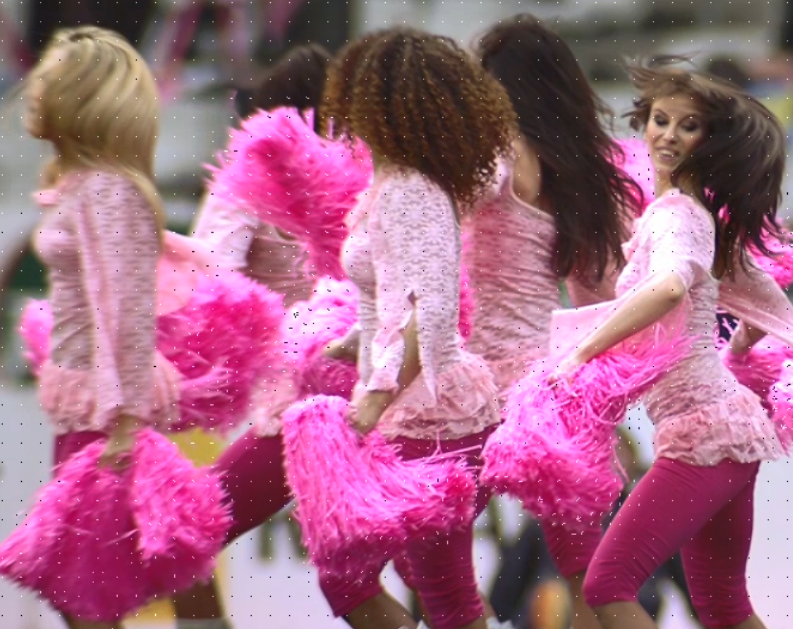
\includegraphics[scale=0.5]{Documeto/1-ElementosTextuais/images/09.png}

    \small
    Extraído dos vídeos fornecidos pelo Professor
\end{figure}

\paragrafo Outra coisa importante em relação a esse vídeo é a distribuição de frames do tipo I, B e P. No pseudo gráfico abaixo é possível identificar pontos de pico. Esses pontos de pico indicam quadros do tipo I. Como a composição do vídeo em slow motion é constituída por menos movimentos, o codec usa os I frames em momentos onde o acúmulo de perdas em relação a outros quadros é muito grande, ou em momentos específicos limitados por flags do arquivo. Repare que na maior parte do tempo, a segunda forma se faz verdadeira, mas há momentos, geralmente nas transições entre cenas, que o codec é obrigado a usar um frame tipo I para evitar maiores perdas.

\paragrafo Além disso, algo interessante ocorre no uso de quadros B e P. A proporção média é de um para um, isto é, um quadro P e um quadro B. Baseado nos nossos testes realizados de forma empírica, momentos de vídeos com maior redundância temporal costumam ter mais frames do tipo B do que a média se comparados a outros trechos do mesmo vídeo. No trecho do filme “The Matrix”, analisado na próxima sessão, há pouca presença de quadros B. No caso do arquivo em slow motion, a relação com a teoria encontrada foi que como a diferença entre um quadro no índice x em relação ao índice x+2 é tão pequena que a taxa de erro da composição também fica muito pequena, tornando viável seu uso do quadro tipo B no índice x+1.

\begin{figure}[H]
    \centering
    \caption{Imagem do vídeo em \textit{slowmotion}}
    \label{fig:imagem10}
    
    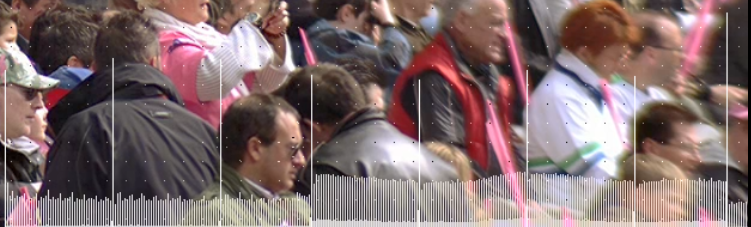
\includegraphics[scale=0.5]{Documeto/1-ElementosTextuais/images/10.png}

    \small
    Extraído dos vídeos fornecidos pelo Professor
\end{figure}

\paragrafo As informações importantes ainda não acabaram. O bitrate acompanha a complexidade da imagem analisada no momento, o que faz todo sentido. Sendo o bitrate a taxa de transferência de dados para a renderização do vídeo, faz sentido que imagens mais complexas exigirem uma maior taxa de transferência. No caso, os trechos mais pesados são os key frames, enquanto a complexidade dos demais é definida pela redundância temporal. Por exemplo, em cenas muito movimentadas, a tendência é que um bitrate maior seja exigido.

\section{Vídeo 2 - Cena Aleatória de The Matrix (1999)}

Boa parte das observações feitas na sessão anterior são válidas nesta sessão. No entanto, essa cena diferencia-se pela forma como foi gravada, que é no tempo normal. Além disso, a cena por si só é extremamente movimentada, com bolsa para lá e pra cá, tiro para todo lado, personagens andando, coadjuvantes morrendo, e zás e zás. Como pode-se perceber, a natureza da cena variou muito de uma análise para outra, assim é mais proveitoso interpretar as diferenças entre os vídeos do que ficar repetindo “mais do mesmo”.

\paragrafo A primeira coisa a se notar é que a imagem do vídeo em questão tem uma paleta de cores na cena mais escura e puxada para o verde se comparado ao vídeo em slow motion. Ou seja, a compressão da imagem é mais perceptível ao olho humano do que se a informação estivesse em regiões mais claras; o que implica na perda de transparência da imagem com mais facilidade. Isso influencia diretamente no bitrate necessário na descompressão. Isto é apenas um detalhe, mas não deixa de ser importante comentar.

\paragrafo Ademais, perceba que a quantidade de informação temporal dessa cena é muito maior do que a do vídeo em \textit{slowmotion}. A Figura \ref{fig:imagem11} demonstra isso com clareza. Nela, há uma vasta quantidade de \textit{motion vercotrs}, o que indica a movimentação das informações na cena, e por sua vez acumula informação. Isso influencia diretamente no bitrate, bem como na presença dos \textit{frames} tipo P e B.

\begin{figure}[H]
    \centering
    \caption{Imagem do filme \textit{The Matrix}}
    \label{fig:imagem11}
    
    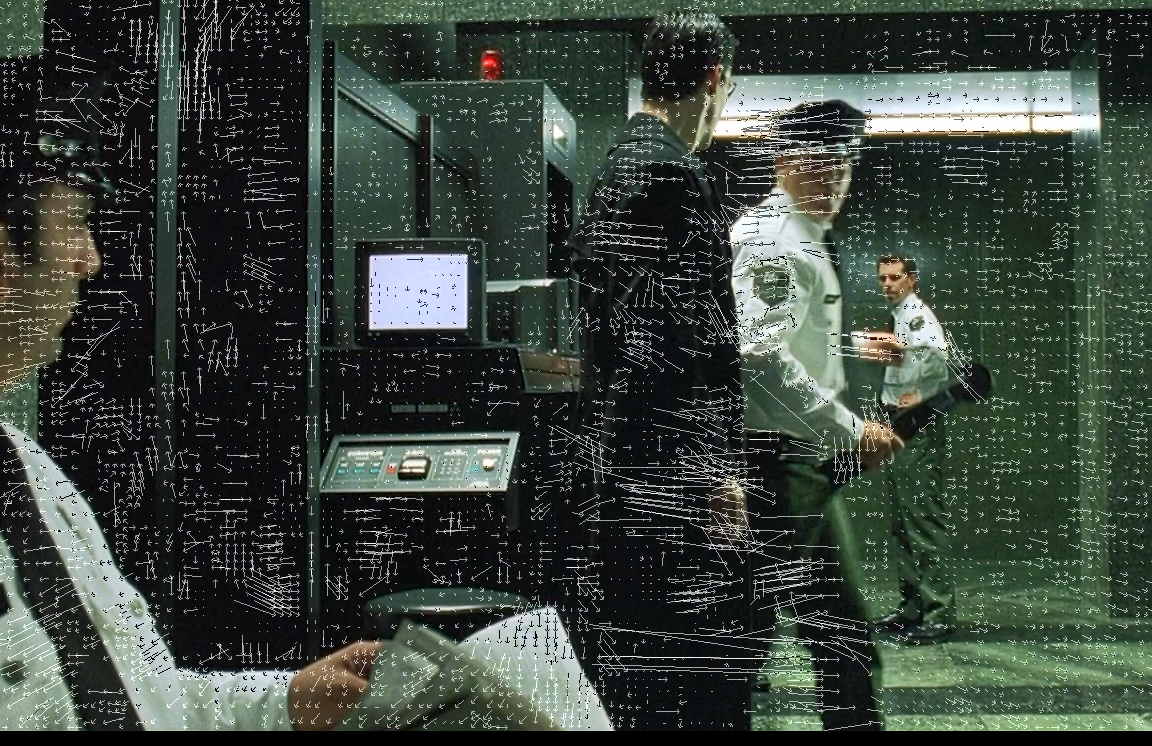
\includegraphics[scale=0.3]{Documeto/1-ElementosTextuais/images/11.png}

    \small
    Extraído dos vídeos fornecidos pelo Professor
\end{figure}

\paragrafo A Figura \ref{fig:imagem12} demonstra quais \textit{frames} o encoder optou por utilizar. Diferente do vídeo em \textit{slowmotion}, o trecho do filme não tão bem comportado. Os \textit{frames} tipo I não estão tão espaçados com a mesma constância que os \textit{frames} do vídeo anterior. Outra coisa que pode ser observadas é que esse tipo de quadro aparece em transições de cena. Além disso, há momentos de constância muito grande de frames tipo P, que são os momentos de uma "onda contínua", enquanto os \textit{frames} tipo B aparecem bem menos, em locais de "altura" menor. 

\begin{figure}[H]
    \centering
    \caption{Imagem do filme \textit{The Matrix}}
    \label{fig:imagem12}
    
    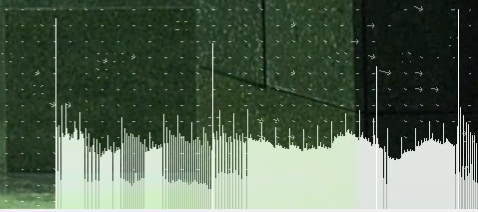
\includegraphics[scale=1]{Documeto/1-ElementosTextuais/images/12.png}

    \small
    Extraído dos vídeos fornecidos pelo Professor
\end{figure}


\section{Vídeo 3 - Último Episódio da Temporada 4 de \textit{Game of Thrones}}
Agora, é o momento de preparar uma pipoca e analisar um episódio longo de uma série mais longa ainda. Como o episódio é muito extenso não iremos comentar ele todo. Ao invés disso, vamos separar trechos interessantes de serem anualizados baseado nos conhecimentos então adquiridos.


\subsection{Um começo caótico}
Primeiramente, vamos analisar a tão famosa abertura da série. No primeiro momento, temos a logo da HBO Entretairement. Essa vinheta inicia-se com um ruído muito intenso, o que aumenta muito o bitrate nesse momento. Como demonstra a Figura \ref{fig:imagem12}, a construção da imagem é de alta complexidade espacial, apesar da pouca complexidade temporal.

\begin{figure}[H]
    \centering
    \caption{Imagens da abertura do episódio citado de \textit{Game of Trhones}}
    \label{fig:imagem13-14-15}
    
    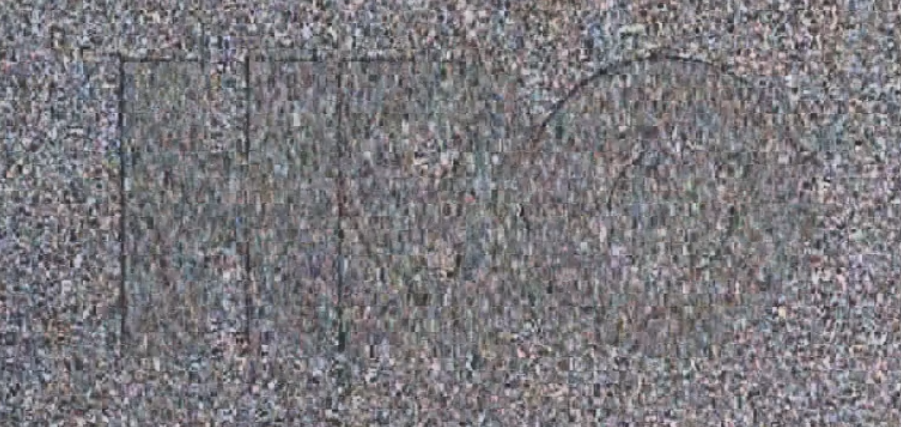
\includegraphics[scale=0.33]{Documeto/1-ElementosTextuais/images/13.png}
    
\includegraphics[scale=0.25]{Documeto/1-ElementosTextuais/images/14.png}

    \small
    Extraído dos vídeos fornecidos pelo Professor
\end{figure}

\paragrafo Então, a abertura da série é exibida e ela tem, de forma geral, uma complexidade bem maior que o resto do episodio, já que o seu \textit{bitrate} foi consideravelmente maior que a média. Isso ocorre devido a dois fatores: primeiro, a complexidade espacial dela é bem grande, com muitas formas bem definidas e regiões com bastante "textura"; a segunda é que a complexidade temporal em toda a cena é bastante constate -- geralmente, uma cena pode ter complexidade temporal alta, mas costuma ser em pontos específicos na tela, ou no cenário ou em um objeto, já na abertura a cena como um todo tem movimento.


\subsection{Cenas escuras}
A Figura \ref{fig:imagem17} traz outra cena do episódio. Enquanto a abertura era bem mais complexa, esse trecho é mais simples. Apesar da correção de movimento ser muito intensa, a forma como a câmera constrói a cena permite muita redundância nas informações.

\begin{figure}[H]
    \centering
    \caption{Imagem do início do episódio citado de \textit{Game of Trhones}}
    \label{fig:imagem17}
    
    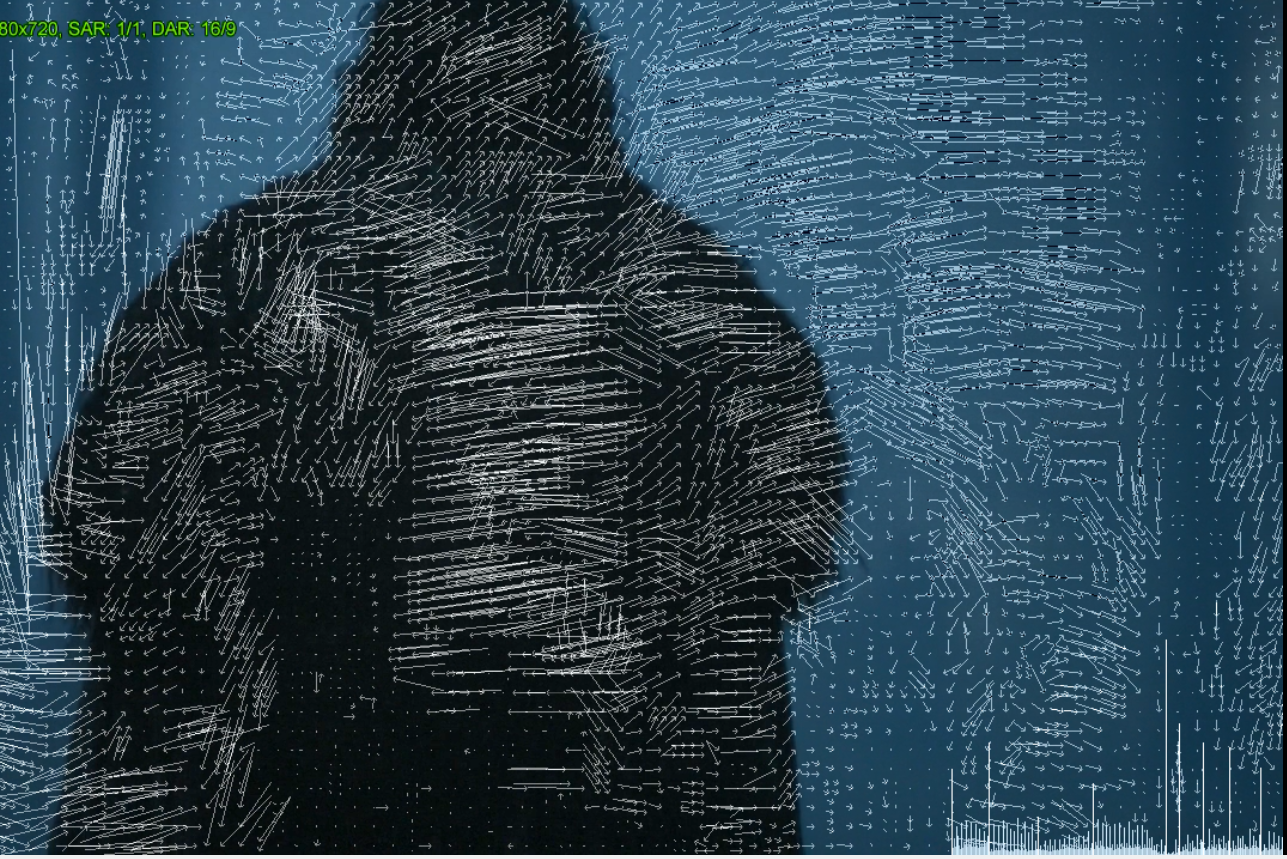
\includegraphics[scale=0.35]{Documeto/1-ElementosTextuais/images/17.png}

    \small
    Extraído dos vídeos fornecidos pelo Professor
\end{figure}

\paragrafo Além disso, cenas que tem um ritmo mais lento tem um gráfico de complexidade mais comportado. Em comparação a cenas mais claras, os artefatos são muito evidentes nos trechos mais escuros, como demonstrado na Figura \ref{fig:imagem18}

\begin{figure}[H]
    \centering
    \caption{Imagem do episódio citado de \textit{Game of Trhones}}
    \label{fig:imagem18}
    
    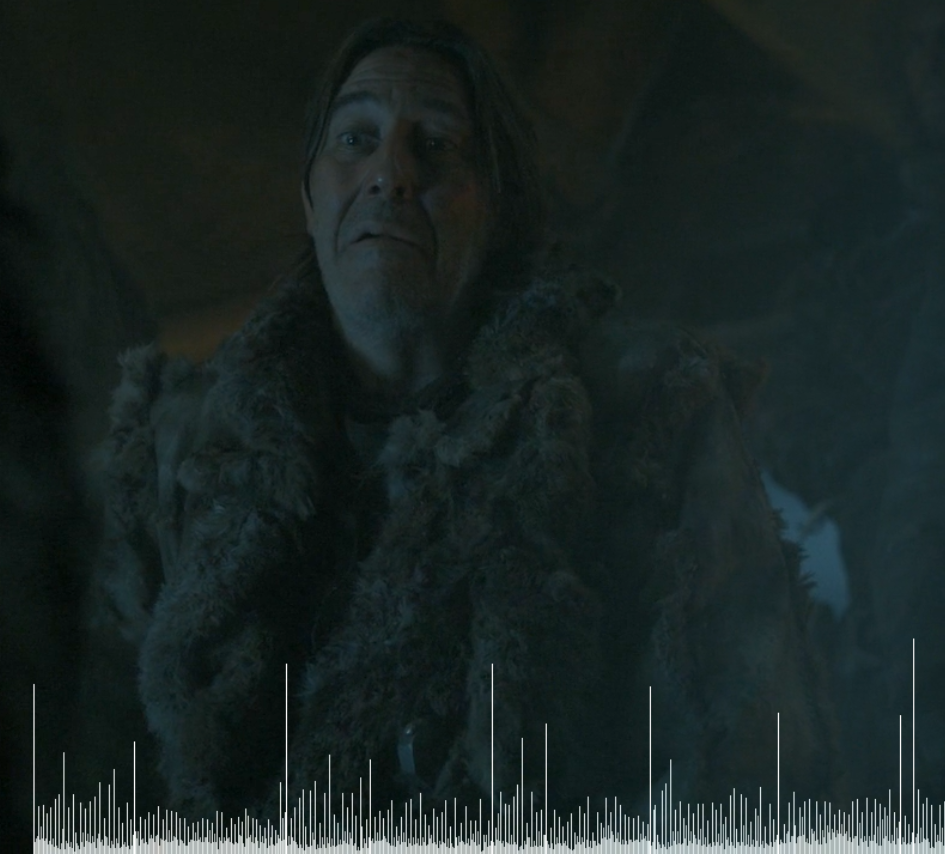
\includegraphics[scale=0.35]{Documeto/1-ElementosTextuais/images/18.png}

    \small
    Extraído dos vídeos fornecidos pelo Professor
\end{figure}


\subsection{Cenas Claras}
Em cenas claras um comportamento semelhante pode ser observado. Regiões mais escuras tem artefatos bastante visíveis, enquanto regiões mais claras são mais transparentes. Além disso, momentos mais calmos apresentam gráficos mais comportados.

\begin{figure}[H]
    \centering
    \caption{Imagem do episódio citado de \textit{Game of Trhones}}
    \label{fig:imagem19}
    
    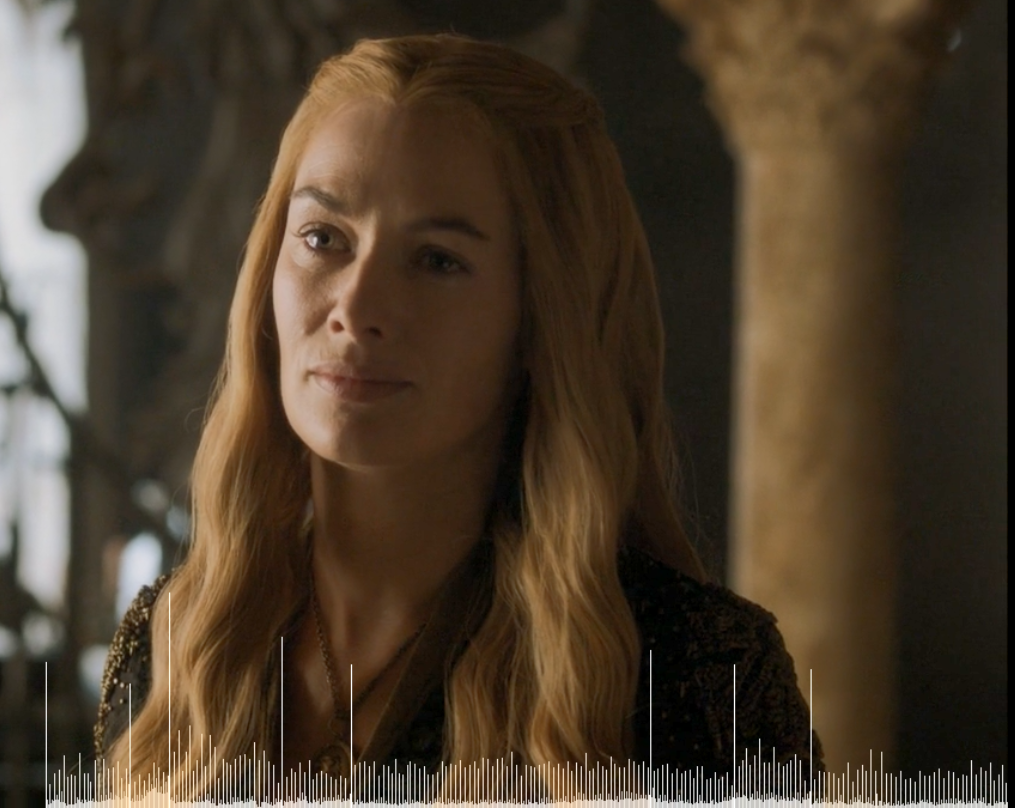
\includegraphics[scale=0.35]{Documeto/1-ElementosTextuais/images/19.png}

    \small
    Extraído dos vídeos fornecidos pelo Professor
\end{figure}

\paragrafo Além disso, é muito interessante perceber como a iluminação artificial e a iluminação natural tem grande influência na percepção dos artefatos e também no comportamento da complexidade da cena. Quando a iluminação é artificial, os artefatos são mais perceptíveis e a transição entre camadas é bem mais suave, valorizando a cena. Além disso, em cenas com iluminação artificial é comum perceber que há uma variância muito brusca na correção de movimento mesmo que as personagens estejam paradas, o que é justificado pelo fato da iluminação artificial "piscar" ao invés de emitir de fato luz.


\begin{figure}[H]
    \centering
    \caption{Imagem do episódio citado de \textit{Game of Trhones} (supostamente em iluminação artificial); a imagem da direita é o exato frame posterior ao frame da esquerda}
    \label{fig:imagem20-21}
    
    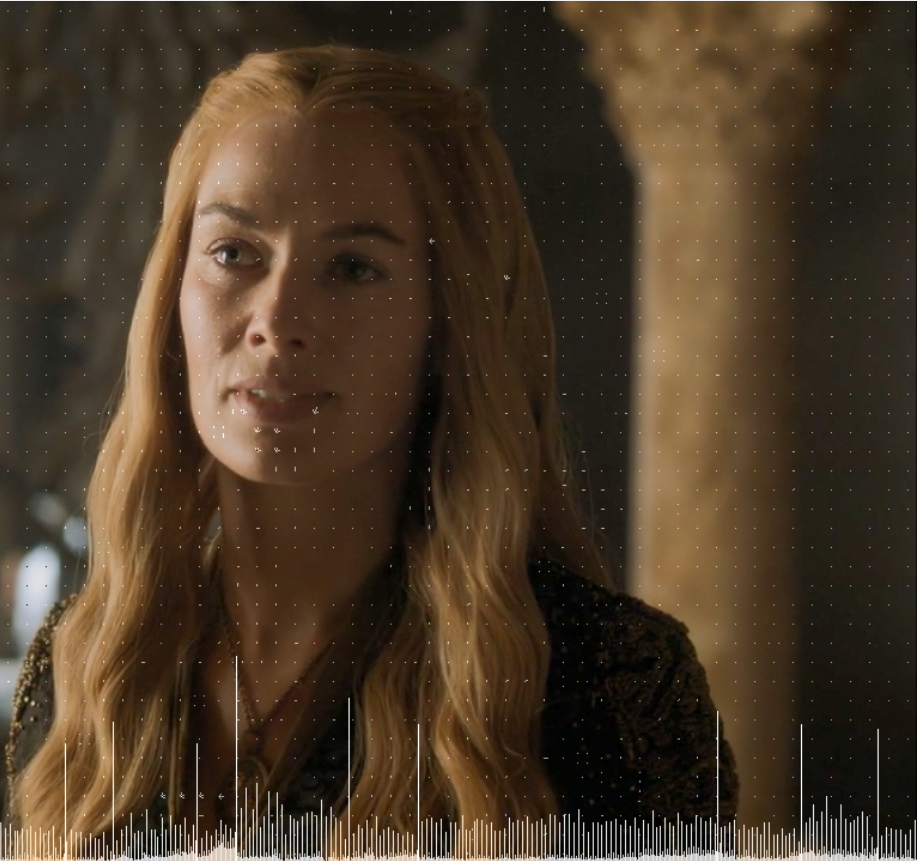
\includegraphics[scale=0.3]{Documeto/1-ElementosTextuais/images/20.png}
    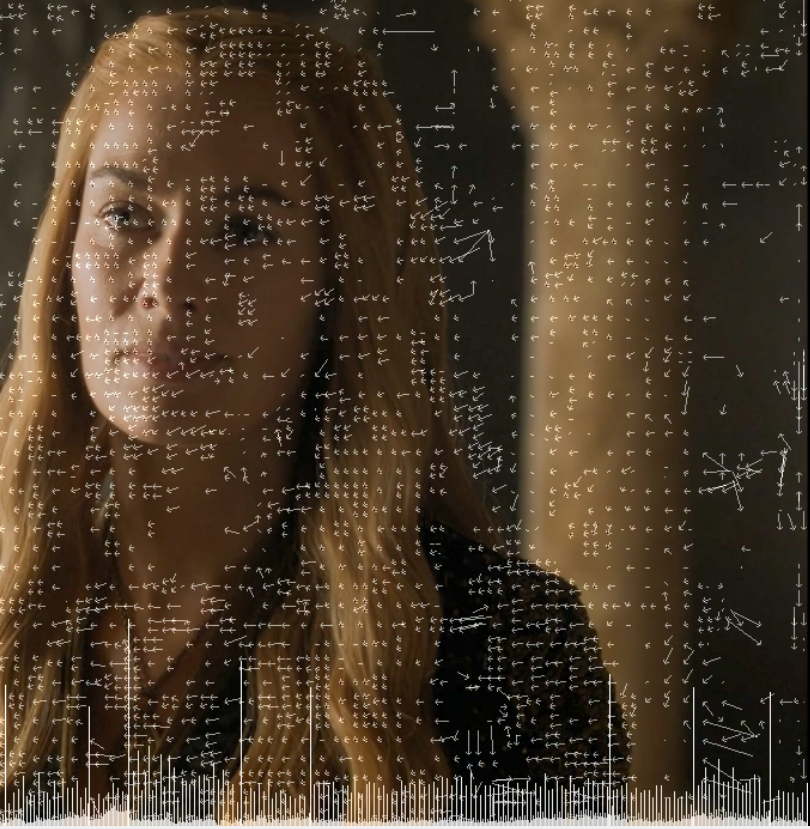
\includegraphics[scale=0.3]{Documeto/1-ElementosTextuais/images/21.png}

    \small
    Extraído dos vídeos fornecidos pelo Professor
\end{figure}


\begin{figure}[H]
    \centering
    \caption{Imagem do episódio citado de \textit{Game of Trhones} (supostamente em iluminação natural); a imagem da direita é o exato frame posterior ao frame da esquerda}
    \label{fig:imagem22-23}
    
    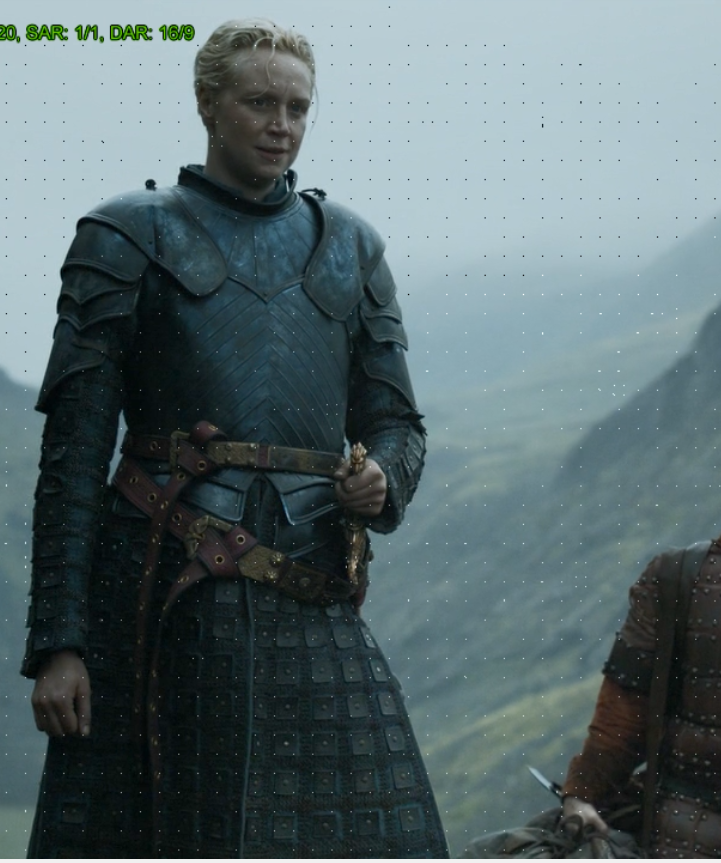
\includegraphics[scale=0.3]{Documeto/1-ElementosTextuais/images/22.png}
    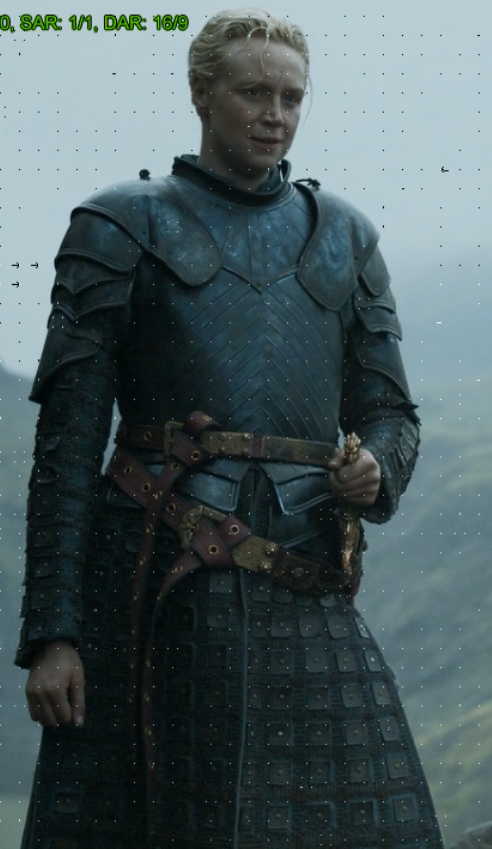
\includegraphics[scale=0.3]{Documeto/1-ElementosTextuais/images/23.png}

    \small
    Extraído dos vídeos fornecidos pelo Professor
\end{figure}

\subsection{Cenas mais calmas com alta complexidade}
Existem cenas que mesmo que sejam bem lentas, a sua complexidade é muito grande. Isso decorre do fato da complexidade temporal ser baixa, mas da espacial ser grande. No episódio, próximo ao final dele, temos uma cena em uma região montanhosa. Como é de se esperar, essa cena tem bastante textura, muitos detalhes e também camadas. Assim, a sua complexidade espacial é bastante alta.

\begin{figure}[H]
    \centering
    \caption{Imagem do episódio citado de \textit{Game of Trhones}}
    \label{fig:imagem24}
    
    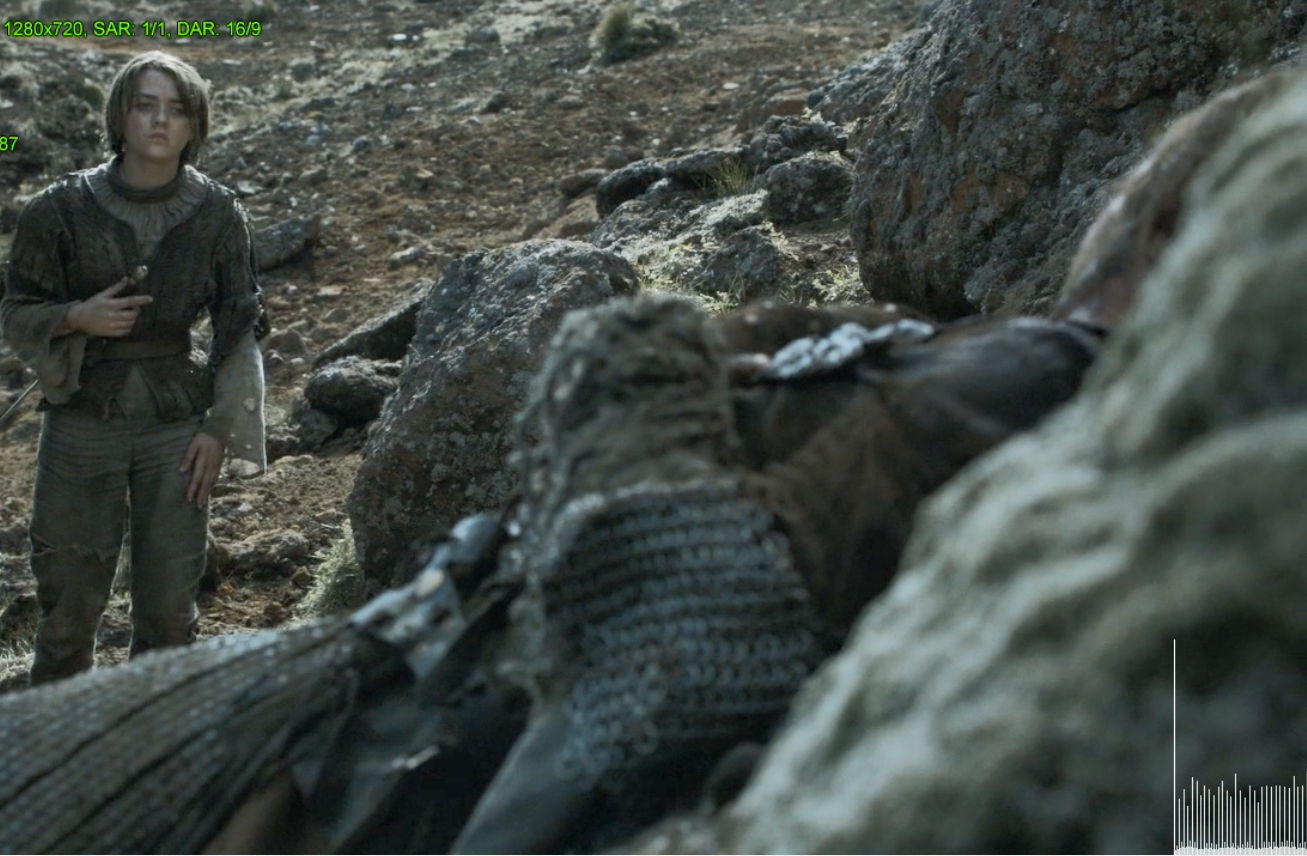
\includegraphics[scale=0.3]{Documeto/1-ElementosTextuais/images/24.png}

    \small
    Extraído dos vídeos fornecidos pelo Professor
\end{figure}